\documentclass[12pt]{article}\usepackage[]{graphicx}\usepackage[]{color}
\usepackage[top=1in,left=1in, right = 1in, footskip=1in]{geometry}

\title{Speed and strength of epidemic intervention}
\author{Jonathan Dushoff, Sang Woo Park}

\usepackage{tabularx}

%% \usepackage{amsmath}
\usepackage{natbib}
\usepackage{hyperref}
\bibliographystyle{chicago}
\date{\today}

\usepackage{bm}

\usepackage{afterpage}
\usepackage{pdflscape}

\newcommand{\etal}{\textit{et al.}}

\newcommand{\comment}[3]{\textcolor{#1}{\textbf{[#2: }\textit{#3}\textbf{]}}}
\newcommand{\jd}[1]{\comment{cyan}{JD}{#1}}
\newcommand{\swp}[1]{\comment{magenta}{SWP}{#1}}

\newcommand{\Rx}[1]{\ensuremath{{\mathcal R}_{#1}}} 
\newcommand{\Ro}{\Rx{0}}
\newcommand{\RR}{\ensuremath{{\mathcal R}}}
\newcommand{\Rhat}{\ensuremath{{\hat\RR}}}
\newcommand{\tsub}[2]{#1_{{\textrm{\tiny #2}}}}

\newcommand{\figref}[1]{Fig.~\ref{fig:#1}}
\newcommand{\figlab}[1]{\label{fig:#1}}
\newcommand{\eqref}[1]{(\ref{eq:#1})}
\newcommand{\eqlab}[1]{\label{eq:#1}}
\begin{document}

\maketitle

\section{To do}

Add a bigger perspective from Eaton and Hallett (SWP can start on that if time). Look also (less important) and Bellan and Dushoff's follow-up to Hollingsworth.

Talk about speed-like and strength-like estimates of an epidemic (e.g., HIV growth rate vs.~measles mean susceptibility) and of an intervention.

\swp{r strategy vs K strategy somewhere}

\section{Introduction}

An epidemic can be described by its \emph{speed} and \emph{strength}.
The speed of an epidemic, often characterized by the exponential growth rate $r$, measures how \emph{fast} an epidemic grows, at the population level. 
The strength of an epidemic, often characterized by the basic reproductive number $\RR_0$, measures how many new cases are caused by a typical \emph{individual} case in a fully susceptible population \citep{anderson1991infectious, diekmann1990definition}.
Knowing the speed and strength of an epidemic allows predictions about the course of the epidemic and the effectiveness of intervention strategies.

Much research has prioritized estimates of the reproductive number, because it has a threshold value, $\RR_0=1$ that determines whether a disease can invade, the level of equilibrium, and the effectiveness of control efforts.
The insight that a case must on average cause at least one new case under good conditions for a disease persist goes back $>100$ years \citep{ross1911prevention};
the idea of averaging by defining a `typical' case was formalized 30 years ago \citep{diekmann1990definition}.
$\RR_0$ is also of interest because it provides a \emph{prima facie} prediction about the total \emph{size} of an epidemic \citep{anderson1991infectious, ma2006generality, miller2012note}.

The study of measles dynamics provides a key example for which the characterization of an epidemic via the basic reproduction number has been successfully applied in controlling the disease.
One of the earliest estimates of the measles $\RR_0$ comes from \cite{anderson1982directly} nearly 40 years ago, who gave a range of $14 - 18$.
This, combined with the mean age of infection (4.6 years) and the mean age of vaccination (2.2 years), allowed them to predict that approximately 96\% of the new birth cohort had to be vaccinated to eradicate measles.
Since then, measles control policies have revolved around targetting this critical vaccination threshold \citep{venczel2003measles, wolfson2007has, takahashi2015reduced}.
\swp{More citations later}
\swp{I think I need to end the paragraph more braodly so that it feels like strength vs speed comparison...}

Like epidemic strength, epidemic speed measures how disease spreads in a population.
Despite the prevailing focus on the basic reproduction number in literature \swp{CITE},
using epidemic speed can be sometimes more effective in characterizing the course of an epidemic and evoluating intervention strategies.
Early in an outbreak, the exponential growth rate can be directly measured from incidence data \citep{chowell2003sars, mills2004transmissibility, nishiura2009transmission, nishiura2010pros, ma2014estimating}, even though the basic reproduction number can be difficult to estimate \citep{weitz2015modeling}.
In these scenarios, we expect control efforts that seek to reduce the epidemic speed to be more effective.
The West African Ebola outbreak in 2014 provides an example for this perspective: 
many researchers tried to estimate the basic reproduction number but the major strategies involved slowing down the epidemic by identifying infected individuals and isolating them \citep{pandey2014strategies}.
Strategies that relied on reducing the epidemic strength (e.g., Ebola vaccine trials) were not implemented until much later and had relatively small effect on controlling the outbreak.
\swp{More citations later}

\swp{Eaton and Hallett?}

Here, we generalize the idea of a threshold for successful intervention by measuring an intervention's ``strength'' on the same scale as the reproductive number. 
We then show that we can likewise measure an intervention's ``speed'', and that there is a duality between the threshold $\RR=1$ and a corresponding minimal intervention strength, and the threshold $r=0$ and a corresponding minimal intervention speed. 
We argue that the historical primacy of $\RR$ over $r$ is partly artificial, and discuss cases where strength provides the better framing for practical disease questions and cases where speed does.

\section{Methods}

\subsection{Epidemic model}

We model disease incidence using the renewal-equation framework, a simple, flexible framework that can cover a wide range of model structures \citep{Champredon2018equivalence}.
In our model, disease incidence at time $t$ is given by:
\begin{equation}
i(t) = \int K(\tau, t) i(t-\tau) d\tau.
\end{equation}
Here, $K(\tau, t)$ is the infection kernel describing how infectious we expect an individual infected $\tau$ time units ago to be in the population.
In general, $K(\tau, t)$ will depend on population characteristics that may change through time $t$ -- notably, the proportion of the population susceptible.
Since we are interested in invasion and control, we will generally neglect changes in $K(\tau, t)$ through time, thus we will assume $K(\tau, t) \equiv K(\tau)$. 
Importantly, this means we are neglecting changes in susceptible proportion through time;
under this assumption, the renewal equation is equivalent to the Von Foerster equations, outlined in \cite{fraser2004factors}.

\subsection{Strength-based decomposition}

\begin{figure}[!t]
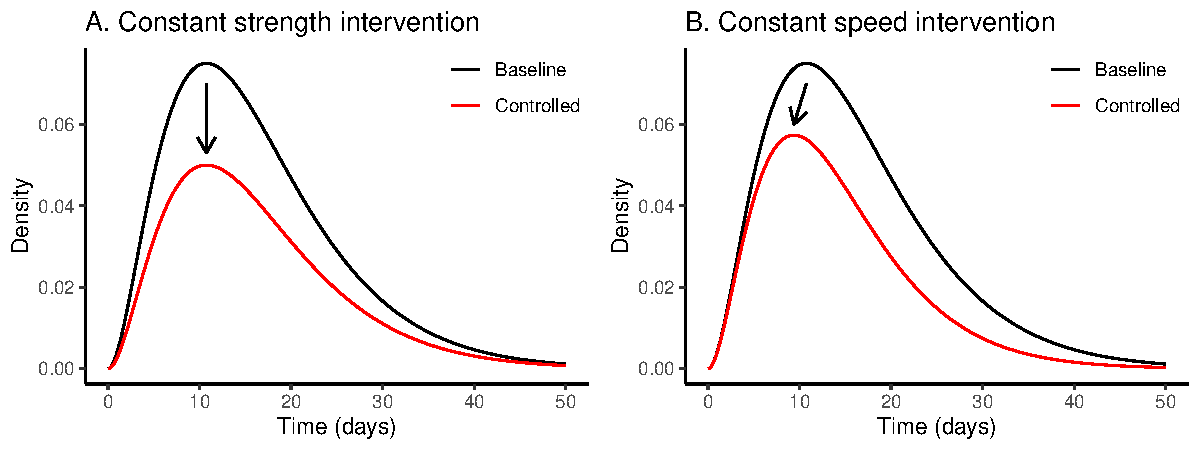
\includegraphics[width=\textwidth]{../figure/constant_intervention.pdf}
\caption{
\textbf{Effects of constant strength and speed intervention on infection kernels.}
Ebola-like gamma infection kernel $K(\tau)$ (mean: 16.2 days, CV: 0.58, and $\RR_0$: 1.5) is shown in black \citep{park2019practical}.
The infection kernel after applying each intervention strategy $\hat K(\tau)$ is shown in red.
(A) A constant strength intervention with $\theta = 1.5$ is applied to Ebola-like infection kernel.
A constant strength intervention reduces the density by a constant proportion: $\hat K(\tau) = K(\tau)/\theta$; the resulting distribution is equivalent to the intrinsic generation-intervla distribution ($\hat K(\tau) = g(\tau)$) when the strength of intervention matches the strength of epidemic ($\theta = \mathcal R$).
(B) A constant speed intervention with $\phi \approx 0.0267\,\mathrm{days}^{-1}$ is applied to Ebola-like infection kernel.
A constant speed intervention reduces the density exponentially: $\hat K(\tau) = K(\tau) \exp(-\phi \tau)$; the resulting distribution is equivalent to the initial backward generation-interval distribution ($\hat K(\tau) = b(\tau)$) when the speed of intervention matches the speed of epidemic ($\phi = r$).
}
\figlab{constant}
\end{figure}

Assuming that the infection kernel $K$ doesn't change with time, we write:
\begin{equation}
	K(\tau) = \RR g(\tau),
	\eqlab{strength}
\end{equation}
where $g(\tau)$ is the ``intrinsic'' generation-interval distribution (giving the relative infectiousness of an average individual as a function of time since infection) \citep{champredon2015intrinsic}. 
Since $g$ is a distribution, it integrates to 1, and the reproduction number $\RR$ is thus the integral of $K$.

Imagine a control measure that proportionally reduces $K$, for example by protecting a fixed fraction of susceptibles (\figref{constant}A). We then have:
\begin{equation}
	\hat K(\tau) = (\RR/\theta) g(\tau).
\end{equation}
Since $g$ is a distribution, the reduction needed to prevent invasion (or to eliminate disease)  is exactly $\theta=\RR$. We call $\theta$ the ``strength'' of the intervention; transmission is interrupted when the strength of the intervention $\theta$ is larger than the strength of spread \RR.

We generalize this idea by allowing an intervention strategy to reduce $K$ by different proportions over the course of an individual infection. We write the post-intervention kernel:
\begin{equation}
	\hat K(\tau) = K(\tau)/L(\tau), 
\end{equation}
where $L(\tau)$ is the average proportional reduction for an individual infected time $\tau$ ago.
The post-intervention reproductive number is thus:
\begin{equation}
	\Rhat = \int \hat K(\tau) d\tau
\end{equation}
This framework generalizes the work of \cite{fraser2004factors} who made parametric assumptions about the shape of $1/L(\tau)$.

We define the strength of the intervention $L$ to be $\theta = \RR/\Rhat$. It is then straightforward to show that $\theta$ is the harmonic mean of $L(\tau)$ weighted by generation-interval distribution:
\begin{equation}
	\theta = 1/\langle 1/L(\tau) \rangle_{g(\tau)}.
\end{equation}
In this more general case, we have again that the disease cannot spread when $\theta \geq \RR$. 

\jd{I'm wondering if we should be diagrammatic about these decompositions. I guess you've seen some of the pictures I show during talks about constant-speed and constant-strength interventions and the relationship to generation intervals.}
\swp{I tried}

\subsection{Speed-based decomposition}

The Euler-Lotka equation allows us to calculate the initial exponential growth rate $r$ of an epidemic given an infection kernel $K$:
\begin{equation}
	1 = \int K(\tau) \exp(-r\tau) d\tau
	\eqlab{euler}
\end{equation}
By analogy with the strength-based factorization \eqref{strength}, we can rewrite \eqref{euler} as a speed-based factorization:
\begin{equation}
K(\tau) = b(\tau)\exp(r\tau)
\end{equation}
Like $g$, $b$ is a distribution: in this case the initial backward generation interval, which gives the distribution of realized generation times (measured from the infectee's point of view) when the disease spreads exponentially \citep{champredon2015intrinsic, britton2019estimation}.

Now imagine an intervention that reduces transmission at a constant hazard rate $\phi$ across the disease generation (\figref{constant}B), for example by identifying and isolating infectious individuals.
We then have:
\begin{equation}
	\hat K(\tau) = K(\tau)\exp(-\phi\tau) = b(\tau)\exp((r-\phi)\tau)
\end{equation}
Since $b$ is a distribution (which integrates to 1), the reduction needed to prevent invasion (or to eliminate disease)  is exactly $\phi=r$. 
We call $\phi$ the ``speed'' of the intervention; transmission is interrupted when the speed of the intervention is faster than the speed of spread.

We generalize this idea by allowing the hazard rate $h(\tau)$ at which $K$ is reduced to vary through time, thus:
\begin{equation}
	\hat K(\tau) = K(\tau) \exp\left(-\int_0^\tau h(\sigma) d\sigma\right)
\end{equation}
The associated post-intervention epidemic speed $\hat r$ is given by:
\begin{equation}
	1 = \int \hat K(\tau) \exp(-\hat r\tau) d\tau.	
\end{equation}
We define the speed of a general intervention to be $\phi = r - \hat r$. 
We can then show that $\phi$ is a (sort of) mean satisfying:
\begin{equation}
	1 = \left\langle \frac{\exp(\phi \tau) }{\exp\left(\int_0^\tau h(\sigma) d\sigma\right)} \right\rangle_{b(\tau)}
\end{equation}
Specifically, the speed $\phi$ is a mean of the hazard $h$ in the sense that an increase (or decrease) in $h$ produces the same sign of change in $\phi$, and if $h$ is constant across the generation then $\phi=h$.

\section{Example: HIV}

\jd{I'd like to be even less detailed about HIV, and maybe do an explicit comparison with measles or Ebola. The idea I'd love to get across is that the two ways of thinking can both be helpful to intuition, and that which one fits better will depend on the disease and on the available data. I will work on making that part explicit.}

In this section, we use both strength- and speed-based decompositions to compare different intervention strategies for the Human immunodeficiency virus (HIV). 
These examples are meant to provide neither precise nor accurate estimates of the effectiveness of intervention strategies; 
instead, we use these examples to demonstrate how strength- and speed-based decompositions can help us better evaluate each control strategy under different scenarios.
In particular, we study how the amount of early HIV transmission affects our decision.

We model the infection kernel of the HIV as a sum of two gamma distributions:
\begin{equation}
K(\tau) = \mathcal R \left(\tsub{p}{early} \tsub{f}{early}(\tau) + (1-\tsub{p}{early}) \tsub{f}{late}(\tau) \right).
\end{equation}
The first component, $\tsub{f}{early}(\tau)$, models early HIV transmission during the acute infection stage.
We assume that $\tsub{f}{early}(\tau)$ has a mean of 3 months \citep{hollingsworth2008hiv} and a shape parameter of 3.
The second component, $\tsub{f}{late}$, models HIV transmission during the asymptomatic stage and the disease stage (after progression to Acquired Immune Deficiency Syndrome (AIDS)).
We assume that $\tsub{f}{late}(\tau)$ has a mean of 10 years \swp{need to cite something and/or change this value} \jd{Happy to use any value you can cite, or to help search} and a shape parameter of 2 (this vaguely approximates the wide generation-interval distribution of the HIV \citep{fraser2004factors}).
Finally, $\tsub{p}{early}$ is the proportion of early HIV transmission.

\begin{figure}[!t]
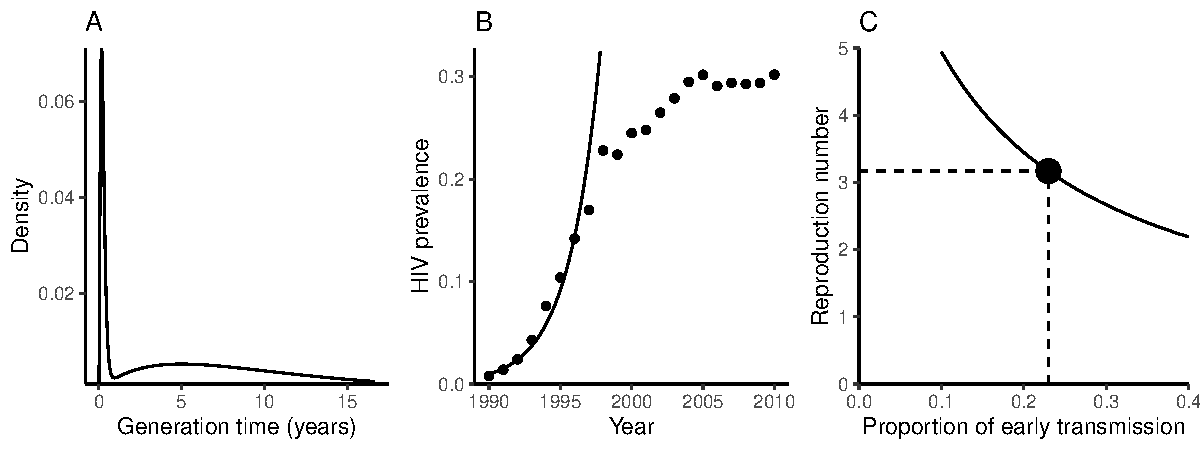
\includegraphics[width=\textwidth]{../figure/HIV.pdf}
\caption{
\textbf{The infection kernel of the HIV.}
A. The infection kernel of the HIV is approximated using a sum of two gamma distributions. We assume that the baseline proportion of early transmission is 23\% \citep{hayes2006amplified}.
B. Time series of HIV prevalence in pregnant women in South Africa, 1990 - 2010 \citep{barron2013eliminating}. The initial exponential growth rate of the HIV is estimated by fitting a straight line to log-prevalence (1990 - 1997) by minimizing the sum of squares.
C. Increasing the proportion of early transmission reduces the estimate of the reproduction number.
}
\figlab{example}
\end{figure}

As our baseline scenario (\figref{example}A), we assume that early transmission is responsible for 23\% of the total transmission \citep{hayes2006amplified}.
Based on the growth rate estimate ($0.452 \textrm{year}^{-1}$; \figref{example}B) from HIV prevalence in pregnant women in South Africa \citep{barron2013eliminating}, our baseline reproduction number is $3.17$.
Further increasing the amount of early transmission reduces the mean generation time, which in turn decreases the reproduction number (\figref{example}C);
therefore, we expect stronger (but not necessarily faster) intervention to be required in order to control the disease when there is more early transmission.

\begin{figure}[!t]
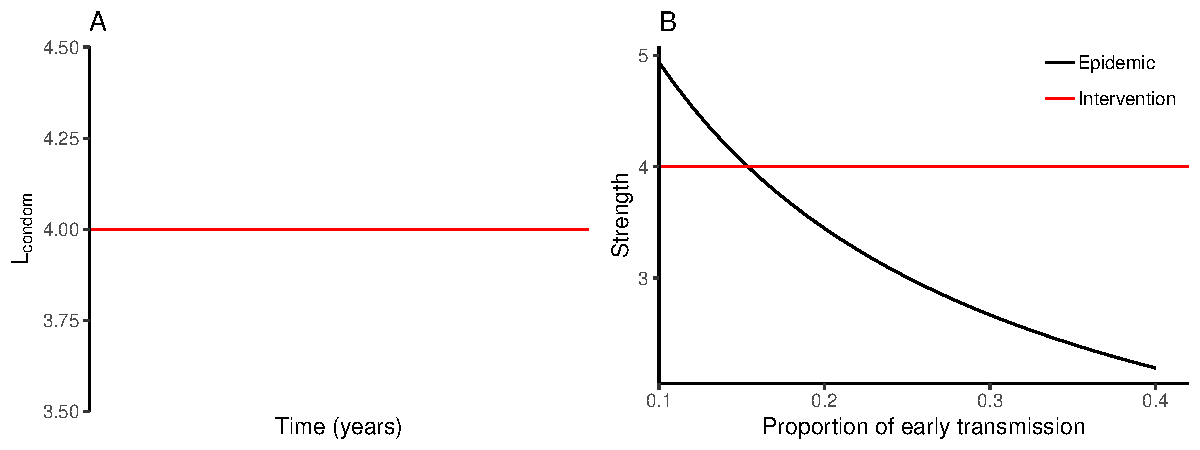
\includegraphics[width=\textwidth]{../figure/condom.pdf}
\caption{
\textbf{Understanding condom intervention using strength-based decomposition.}
A. Condom use is thought to reduce probability of transmission by a similar factor throughout the course of infection; thus the proportional reduction $L$ due to condom use is constant across the course of infection. 
B. The estimated amount of early transmission affects estimated strength of the epidemic but not of a condom-based intervention.
}
\figlab{condom}
\end{figure}

We consider a condom intervention that reduces HIV transmission by approximately 75\% at the population level. \jd{I'm not sure we need to be worried about weller2002condom, nor about population vs.~individual level effects. Many estimates of efficacy are higher than 80\%, and it's certainly possible to imagine an intervention that involves education about condom use.}
Assuming that condoms act as a physical barrier, and that condom use will on average remain roughly constant through time, it is reasonable to model the proportional reduction in transmission due to condom use as constant across the course of infection: $\tsub{L}{condom} = 1/(1-0.75) = 4$  (\figref{condom}A).
The estimated strength of such an intervention is simply the average of $L$: $\theta=4$, whereas the estimated strength of the epidemic increases as the proportion of early transmission decreases (\figref{condom}B).
Thus, the predicted effectiveness of the condom intervention will depend strongly on our estimate of the importance of early transmission: if early transmission is low, we expect disease spread to be too strong to be controlled completely by our intervention. 

\begin{figure}[!t]
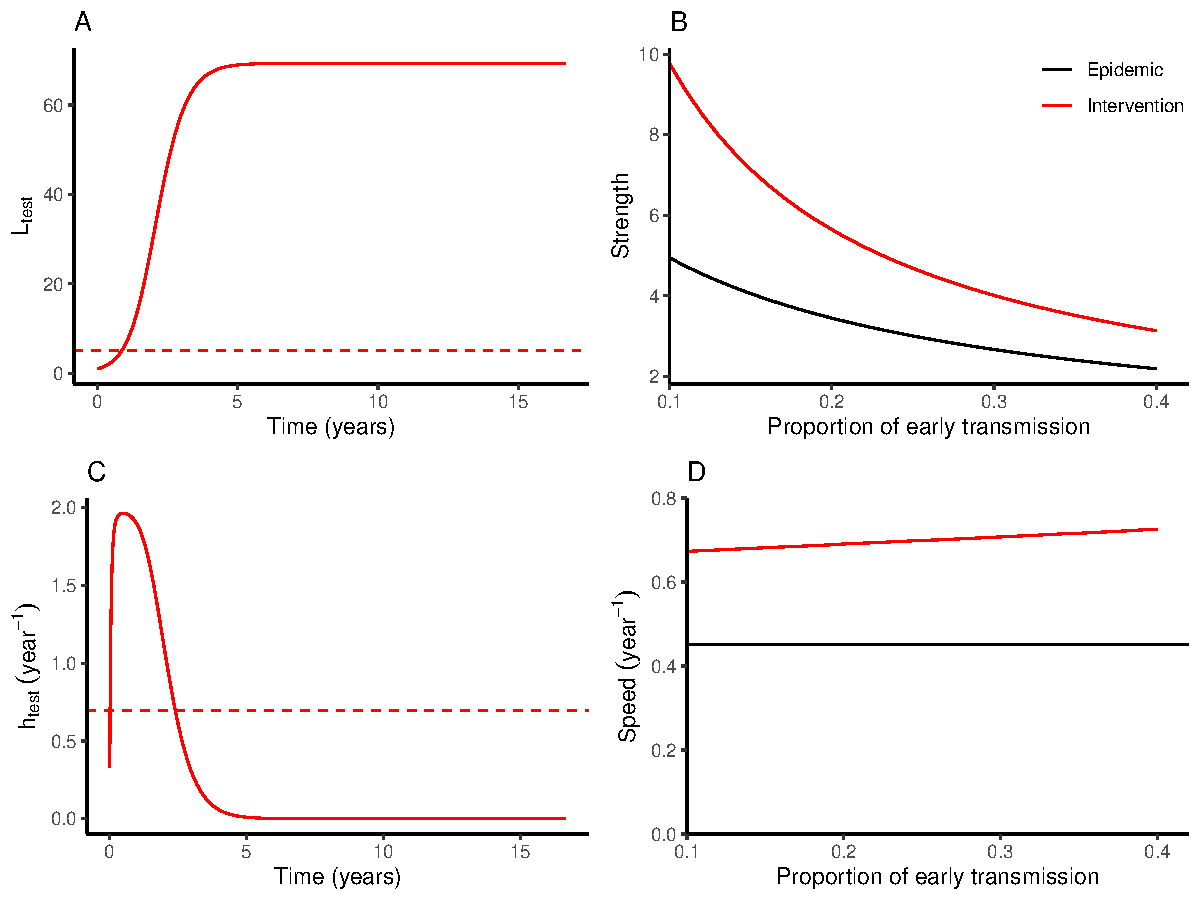
\includegraphics[width=\textwidth]{../figure/test_and_treat.pdf}
\caption{
\textbf{Understanding test-and-treat intervention using strength- and speed-based decomposition.}
A. Test-and-treat intervention $\tsub{L}{test}$ starts at 1 and saturates after about 5 years.
B. Increasing the amount of early transmission decreases the strength of an epidemic as well as the strength of test-and-treat intervention.
C. Hazard rate $\tsub{h}{test}$ of test-and-treat intervention $\tsub{L}{test}$ peaks and plateaus very quickly and reaches zero after about 5 years.
D. The amount of early transmission has no effect on the speed of an epidemic and small effect on the speed of intervention.
We assume $\tsub{L}{test}(\tau) = \exp\left(\int_0^\tau h(\sigma) d\sigma \right)$ and $h(\tau) = \tsub{h}{max} (1 - \exp(- K f(\tau)))$, where $f(\tau)$ is a gamma probability density function with a mean of $12$ months and a shape parameter of 2, $K = 4/\max(f(\tau))$, and $\tsub{h}{max} = 1/6$.
}
\figlab{test}
\end{figure}

On the other hand, consider a test-and-treat strategy in which infected individuals are identified and put to clinical care (e.g., antiretroviral therapy).
We assume that the rate of identification and removal is initially constant. Thus, the proportion continuing to transmit declines exponentially, and the effect of intervention $\tsub{L}{test}$ increases exponentially.
\jd{Can you remind me the functional form that we used?}
However, we assume removal eventually saturates, to account for the effects of people who avoid identification, persistent treatment failures, and the possibility of rare transmission even under effective treatment
\jd{I'm not sure the advantage of the tsub; I kind of feel like we can communicate in context without subscripts.} (\figref{test}A).
Under this assumption, the strength of intervention decreases as the proportion of early transmission increases but is always higher than the epidemic strength; however, it is unclear why this should be the case. \jd{Ref Eaton}

Using the speed-based decomposition allows us to understand the problem much more clearly.
The hazard rate $\tsub{h}{test}$ of this intervention starts at 0 (because infected individuals don't have a way to know that they have HIV when they're infected) but peaks very fast (because individuals are actively getting tested and treated); 
the hazard rate goes down soon after the peak and reaches 0 after about 5 years because infected individuals who have access to medical care would have been identified within the first 5 years or so.
The speed of epidemic stays constant regardless of the proportion of the early transmission because epidemic speed corrresponds to the observed growth rate.
The speed of intervention stays roughly constant but slightly increases as proportion of early transmission increases because the subpopulation that the intervention fails to reach become relatively more important if late transmission is more important.

This framework provides an intuitive underpinning for the originally surprising result of Eaton: the effectiveness of test-and-treat interventions should not depend much on the proportion of early transmission because early transmission has no effect on the estimated speed of the epidemic, and little on the estimated speed of the intervention.

\section{Discussion}



\bibliography{speedstrength}

\end{document}
